\documentclass[12pt]{article}

% ---------- Page & Font ----------
\usepackage[a4paper,margin=1in]{geometry}
\usepackage{times}

% ---------- Encoding Fix ----------
\usepackage[T1]{fontenc}
\usepackage[utf8]{inputenc}

% ---------- Useful Packages ----------
\usepackage[hidelinks]{hyperref}
\usepackage{cite}
\usepackage{graphicx}
\usepackage{amsmath,amssymb,amsfonts}
\usepackage{placeins} % FIXES figure placement issue

\begin{document}

% ---------------- Title Block ----------------
\begin{center}

    {\fontsize{17pt}{20pt}\selectfont
        \textbf{Identity Document Image Tampering Detection Using Multistream Texture, Frequency, and Noise Analysis}
    }\\[1.2cm]

    {\fontsize{13pt}{16pt}\selectfont
    Abhishek Panthee$^{1}$, Kiran Paudel$^{2}$, Raman Shrestha$^{3}$}\\[0.4cm]

    {\fontsize{8pt}{10pt}\selectfont
    $^{1}$Department of Electronics and Computer Engineering, Institute of Engineering Thapathali Campus, Kathmandu, Nepal\\
    $^{2}$Department of Electronics and Computer Engineering, Institute of Engineering Thapathali Campus, Kathmandu, Nepal\\
    $^{3}$Department of Electronics and Computer Engineering, Institute of Engineering Thapathali Campus, Kathmandu, Nepal\\
    }

\end{center}

% ---------------- Introduction ----------------
\section{Introduction}

In today's digital ecosystem, identity verification systems rely heavily on official identity documents such as national identity cards, passports, visas, and residence permits. Identity document images are widely used in online verification, e-government services, financial applications, and border control systems. With the increased digitization of these processes, identity document images are frequently shared through smartphones, scanners, and online submission platforms, which has significantly increased the risk of document forgery and identity fraud.

Advances in image-editing software and generative artificial intelligence have enabled malicious actors to manipulate identity document images with high visual realism. Sensitive information such as names, identification numbers, dates of birth, nationality, and facial photographs can be altered while preserving overall visual consistency. Common tampering operations include copy-move, splicing, erasing, and generation-based editing, targeting textual fields, facial regions, background textures, and security elements.

Unlike natural images, identity documents exhibit structured layouts, repetitive background textures, uniform typography, and standardized visual elements. Tampered regions are typically small and localized, making them difficult to detect through simple visual inspection. Furthermore, secondary editing operations such as JPEG recompression, resizing, scanning artifacts, and camera noise can further suppress forensic traces, increasing the likelihood of undetected forgeries.

Therefore, effective identity document tampering detection requires methods that go beyond RGB appearance and incorporate complementary forensic cues such as texture inconsistencies, frequency-domain artifacts, and noise distribution irregularities.

% ---------------- Objectives ----------------
\section{Objectives}

The primary objectives of this research are as follows:

\begin{enumerate}
    \item To develop a robust identity document image tampering detection framework capable of accurately \textbf{localizing tampered regions} at the pixel level under diverse manipulation strategies and secondary editing operations.
    \item To design a reliable \textbf{binary classification system} that distinguishes between authentic and tampered identity document images by leveraging multi-domain forensic features.
\end{enumerate}

% ---------------- Literature Review ----------------
\section{Literature Review}

Research on identity document image tampering detection intersects with document image forensics, identity fraud analysis, and tampered text localization.

\subsection{Document Image Tampering Detection Using Visual and Frequency Domain Cues}

Qu et al.~\cite{Qu2023DocTamper} proposed a document tampering detection framework that integrates RGB features with frequency-domain representations derived from JPEG artifacts. Their work demonstrated that RGB-only approaches are insufficient for detecting visually consistent tampering, particularly under image compression.

\subsection{Identity Document Tampering Detection Using Texture Understanding and Multistream Networks}

Wang et al.~\cite{Wang2025Identity} introduced a multistream network architecture that jointly models texture, frequency-domain, and noise features for identity document tampering detection. By exploiting document-specific background textures and multiscale feature fusion, their method showed strong robustness against secondary editing operations.

\subsection{Open-Set Tampered Text Detection in the Era of Generative AI}

Qu et al.~\cite{Qu2025OSTF} explored tampered text detection under open-set conditions to address unseen forgery methods introduced by generative AI. Their findings highlight the importance of texture-based anomaly perception for generalization, which is relevant to future identity document forgery scenarios.

% ---------------- Research Gaps ----------------
\section{Research Gaps}

Despite significant progress in document image forensics, several limitations existed in prior approaches when applied to identity document tampering detection.

\subsection{Single-Domain Feature Dependence}
Many earlier methods relied predominantly on RGB-domain features, which lack sensitivity to subtle texture and frequency inconsistencies introduced by small-scale identity document tampering.

\subsection{Limited Robustness to Secondary Editing}
Most existing models were trained on single-edited images and exhibited degraded performance when exposed to recompression, scanning, or re-photographing operations.

\subsection{Neglect of Identity Document-Specific Characteristics}
Generic document tampering detectors often ignore identity document-specific properties such as structured layouts, background security textures, and uniform typography.

\subsection{Weak Multi-Domain Feature Fusion}
Although some studies incorporated frequency or noise features, fusion strategies were often shallow or single-scale, limiting their effectiveness for detecting localized tampering.

\subsection{Lack of Realistic Identity Document Tampering Datasets}
The absence of identity document-focused datasets with diverse tampering types and detailed annotations hindered robust evaluation and real-world deployment.

% ---------------- Dataset Description ----------------
\section{Dataset Description}

\subsection{ID Card Fraud Detection Dataset}

To evaluate the proposed identity document image tampering detection framework, we employ the \textbf{ID Card Fraud Detection Dataset}, a large-scale synthetic dataset designed to simulate realistic identity document tampering scenarios. The dataset is constructed to support both \textbf{pixel-level tampering localization} and \textbf{image-level authenticity classification}.

The dataset consists of a total of \textbf{47,838 identity document images}, including \textbf{5,979 authentic samples} and \textbf{35,873 tampered samples}. All images follow a standardized Greek national ID card layout, ensuring consistent document structure, typography, background texture patterns, and facial region placement. The dataset is synthetically generated to simulate real-world ID cards while avoiding privacy and ethical concerns associated with real personal data.

\subsection{Tampering Categories}

The dataset covers six representative tampering types commonly encountered in identity document forgery:

\begin{itemize}
    \item Copy-and-move tampering
    \item Face morphing tampering
    \item Face replacement tampering
    \item Combined tampering
    \item Inpaint-and-rewrite tampering
    \item Crop-and-replace tampering
\end{itemize}

Authentic samples contain no manipulation, while each tampered sample belongs to exactly one category.

\subsection{Annotation Strategy}

The dataset provides structured annotation information in JSON format. Image-level annotations indicate whether an identity document is \textbf{authentic or tampered}, while region-level annotations specify the spatial locations of manipulated areas.

Pixel-level tampering masks are constructed as the \textbf{union of all annotated tampered regions}, enabling comprehensive supervision for learning localized tampering patterns across different document components.

\subsection{Dataset Statistics}

Table~\ref{tab:dataset_statistics} summarizes the statistical distribution of the ID Card Fraud Detection Dataset.

\begin{table}[h]
    \centering
    \caption{Statistical Summary of the ID Card Fraud Detection Dataset}
    \label{tab:dataset_statistics}
    \begin{tabular}{|l|l|c|}
        \hline
        \textbf{Category}              & \textbf{Description} & \textbf{Number of Images} \\
        \hline
        Authentic Samples              & Genuine ID cards     & 5,979                     \\
        Fraud Type 1                   & Copy-and-move        & 5,979                     \\
        Fraud Type 2                   & Face morphing        & 5,979                     \\
        Fraud Type 3                   & Face replacement     & 5,979                     \\
        Fraud Type 4                   & Combined tampering   & 5,979                     \\
        Fraud Type 5                   & Inpaint and rewrite  & 5,979                     \\
        Fraud Type 6                   & Crop and replace     & 5,978                     \\
        \hline
        \textbf{Total Tampered Images} & --                   & \textbf{35,873}           \\
        \textbf{Total Images}          & --                   & \textbf{47,838}           \\
        \hline
    \end{tabular}
\end{table}

\subsection{Dataset Characteristics and Suitability}

All images are stored in PNG format and represented in the RGB color space. The dataset preserves the structured nature of identity documents, including fixed layouts, uniform fonts, and repetitive background textures. These characteristics are particularly important for learning subtle inconsistencies in texture, frequency-domain artifacts, and noise distributions introduced by tampering operations.

By encompassing diverse tampering strategies and providing both image-level and region-level supervision, the ID Card Fraud Detection Dataset is well suited for evaluating identity document tampering detection methods that jointly perform \textbf{tampering localization and binary classification}.

\section{Data Preprocessing}

This work utilizes the \textit{ ID Card Fraud Detection Dataset}, a large-scale synthetic document fraud dataset containing both genuine and manipulated driver's license images. The dataset includes multiple categories of fraud such as copy--move, face morphing, face replacement, inpainting with text rewriting, and combined manipulation attacks, along with detailed metadata and bounding-box annotations.

\subsection{Data Organization and Label Mapping}

The dataset is organized into multiple directories based on fraud type. These directories include:

\begin{itemize}
    \item \path{fraud1_copy_and_move}
    \item \path{fraud2_face_morphing}
    \item \path{fraud3_face_replacement}
    \item \path{fraud4_combined}
    \item \path{fraud5_inpaint_and_rewrite}
    \item \path{fraud6_crop_and_replace}
\end{itemize}

A separate \path{positive} directory contains genuine (non-tampered) images. Each image is assigned a binary label, where genuine images are labeled as $0$ and fraudulent images are labeled as $1$.

Detailed fraud annotations are provided in JSON format under the \path{meta/detailed_with_fraud_info} directory. These annotation files contain manipulation-specific labels and bounding-box coordinates for forged regions, including face regions and ghost artifact regions. During preprocessing, the JSON files are parsed and aligned with their corresponding images using consistent filename matching.
\subsection{Image Normalization}

All images are converted to the RGB color space to ensure consistency across different formats (PNG and JPG). Images are resized to a fixed spatial resolution of $512 \times 512$ pixels using bilinear interpolation while preserving the aspect ratio through padding when necessary. Before feeding images into the deep learning model, a standard image normalization
pipeline is applied to reduce illumination variations, stabilize training, and ensure
numerical consistency across samples.

\begin{enumerate}
    \item \textbf{Color Space Conversion:}
          Each input image $I$ is converted to the RGB color space (if not already in RGB)
          to maintain consistency across all samples.

    \item \textbf{Resizing:}
          All images are resized to a fixed spatial resolution of $H \times W$ using bilinear
          interpolation:
          \[
              I \in \mathbb{R}^{H_0 \times W_0 \times 3} \rightarrow I' \in \mathbb{R}^{H \times W \times 3}
          \]

    \item \textbf{Pixel Value Scaling:}
          Pixel intensity values are normalized from the original range $[0, 255]$ to
          $[0, 1]$:
          \[
              I_s = \frac{I'}{255}
          \]

    \item \textbf{Mean Subtraction and Standard Deviation Normalization:}
          Each color channel is normalized independently using dataset-level mean
          $\boldsymbol{\mu}$ and standard deviation $\boldsymbol{\sigma}$:
          \[
              I_n^{(c)} = \frac{I_s^{(c)} - \mu^{(c)}}{\sigma^{(c)}}, \quad c \in \{R, G, B\}
          \]
          where $\mu^{(c)}$ and $\sigma^{(c)}$ denote the mean and standard deviation of
          channel $c$ computed over the training set.

    \item \textbf{Final Normalized Input:}
          The resulting normalized image $I_n$ is used as input to the network:
          \[
              I_n \in \mathbb{R}^{H \times W \times 3}
          \]
\end{enumerate}

This normalization process ensures stable gradient propagation, faster convergence,
and improved generalization performance during training.


\subsection{Region-of-Interest Processing}

For images with available bounding-box annotations, the annotated face regions and artifact regions are extracted and stored as region-of-interest (RoI) samples. These RoIs are used to guide supervised learning for localization-based tampering detection. For models requiring pixel-level supervision, bounding boxes are converted into binary mask representations, where tampered regions are marked as foreground and the remaining regions as background.

\subsection{Handling Class Imbalance}

Since the dataset contains a significantly larger number of fraudulent images compared to genuine images, class imbalance is addressed during preprocessing. This is achieved by applying class-aware sampling during training, ensuring balanced exposure of genuine and tampered samples in each mini-batch.

\subsection{Data Augmentation}

To improve model generalization and robustness to real-world distortions, data augmentation is applied exclusively to the training set. The augmentation pipeline includes random horizontal flipping, small-angle rotation ($\pm15^\circ$), brightness and contrast adjustment ($\pm20\%$), Gaussian noise injection, and JPEG recompression with varying quality factors. No augmentation is applied to the validation or test sets to preserve evaluation integrity.

\subsection{Train--Validation Split}

The dataset is divided into training and testing subsets using an $80{:}20$ split at the image level, ensuring that no identity overlap exists between the two subsets. Metadata and annotation files are split accordingly to prevent data leakage and to ensure fair evaluation.

Through this preprocessing pipeline, the dataset is transformed into a clean, standardized, and well-annotated form suitable for training deep learning models for document fraud and tampering detection.

\clearpage

\section{Proposed Model Architecture}

\begin{figure}[!ht]
    \centering
    \IfFileExists{architecture.png}{%
        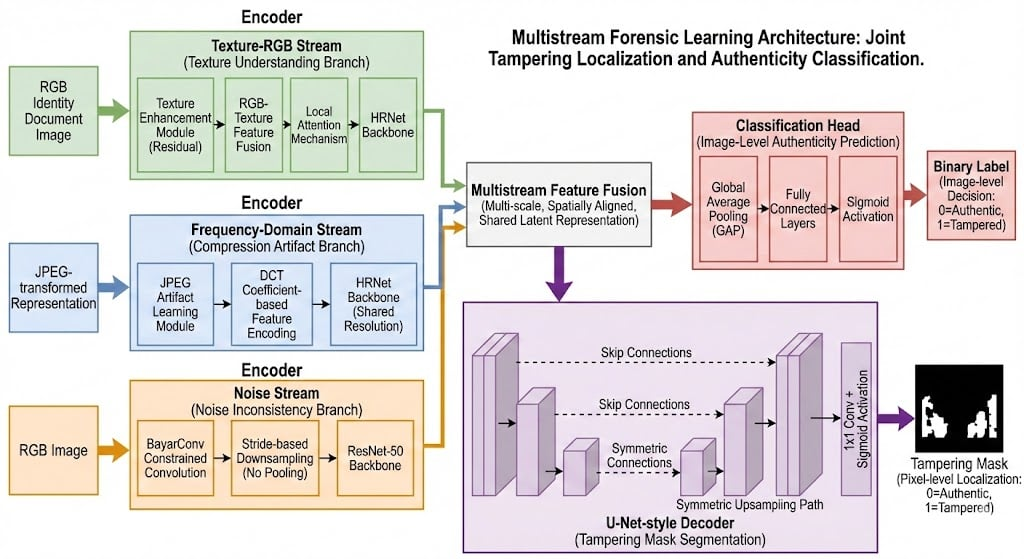
\includegraphics[width=\textwidth]{architecture.png}%
    }{%
        \fbox{Missing image: architecture.png}%
    }
    \caption{Proposed multistream forensic learning architecture for identity document image tampering detection. Parallel texture--RGB, frequency-domain, and noise streams extract complementary features. A U-Net--style decoder enables pixel-level tampering localization, while a classification head performs image-level authenticity prediction.}
    \label{fig:multistream_unet_architecture}
\end{figure}

\FloatBarrier

\subsection{Multistream Encoder}

The encoder comprises three parallel feature extraction branches, each designed to capture complementary forensic cues.

\subsubsection{Texture--RGB Stream}

The texture--RGB stream is responsible for modeling background texture irregularities and subtle visual inconsistencies specific to identity documents. A texture enhancement module extracts residual texture information, which is further refined using a local attention mechanism guided by high-level semantic features. The extracted texture features are fused with RGB features and processed using a High-Resolution Network (HRNet) backbone.

\subsubsection{Frequency-Domain Stream}

The frequency-domain stream focuses on detecting compression artifacts and frequency discontinuities caused by secondary editing operations. JPEG-transformed representations of the input image are used to extract DCT-based features, which are then processed using an HRNet backbone to preserve multi-scale spatial consistency.

\subsubsection{Noise Stream}

The noise stream captures noise distribution inconsistencies introduced during tampering. A constrained Bayar convolution suppresses semantic content while amplifying noise residuals. Feature extraction is performed using a ResNet-50 backbone without pooling layers to avoid loss of noise information.

\subsection{Multistream Feature Fusion}

Features extracted from the three streams are spatially aligned and fused using a multi-scale feature fusion module. This fusion integrates texture, frequency, and noise cues into a unified latent representation, serving as the shared encoder output for downstream tasks.

\subsection{U-Net Decoder for Tampering Segmentation}

To enable pixel-level tampering localization, a U-Net–style decoder is attached to the fused encoder representation. The decoder employs progressive upsampling and skip connections from corresponding encoder stages to recover fine-grained spatial details. A final $1\times1$ convolution followed by a sigmoid activation produces a binary tampering mask, where foreground pixels correspond to manipulated regions.

\subsection{Classification Head}

In parallel with segmentation, an image-level classification head is introduced to determine document authenticity. Global average pooling is applied to the fused encoder features, followed by fully connected layers and a sigmoid activation to output a binary tampering probability.

\subsection{Multi-Task Learning Objective}

The model is trained end-to-end using a multi-task loss function that jointly optimizes segmentation and classification objectives:

\[
    \mathcal{L}_{total} = \lambda_{seg}\mathcal{L}_{seg} + \lambda_{cls}\mathcal{L}_{cls},
\]

where $\mathcal{L}_{seg}$ denotes the segmentation loss and $\mathcal{L}_{cls}$ denotes the classification loss. This joint optimization enables the model to learn both localized and global tampering cues.


\section{Evaluation Metrics}

To quantitatively evaluate the performance of the proposed tampered image detection
and localization framework, standard classification metrics are employed. These
metrics assess both the correctness of predictions and the robustness of the model
under varying decision thresholds.

\subsection{Confusion Matrix}

The confusion matrix summarizes the prediction results by comparing the predicted
labels with the ground-truth labels. It consists of four fundamental components:

\begin{itemize}
    \item \textbf{True Positives (TP):} Tampered samples correctly identified as tampered.
    \item \textbf{True Negatives (TN):} Authentic samples correctly identified as authentic.
    \item \textbf{False Positives (FP):} Authentic samples incorrectly classified as tampered.
    \item \textbf{False Negatives (FN):} Tampered samples incorrectly classified as authentic.
\end{itemize}

\begin{table}[h]
    \centering
    \caption{Confusion Matrix for Tampering Detection}
    \begin{tabular}{c|c|c}
        \hline
        \textbf{Ground Truth} & \textbf{Predicted Tampered} & \textbf{Predicted Authentic} \\
        \hline
        Tampered              & TP                          & FN                           \\
        Authentic             & FP                          & TN                           \\
        \hline
    \end{tabular}
\end{table}

The confusion matrix provides a complete view of classification behavior and serves
as the basis for computing higher-level evaluation metrics.

\subsection{Precision, Recall, and F1-Score}

Using the confusion matrix components, precision and recall are defined as:
\[
    \text{Precision} = \frac{TP}{TP + FP}
\]
\[
    \text{Recall} = \frac{TP}{TP + FN}
\]

The \textbf{F1-score}, which balances precision and recall, is computed as:
\[
    \text{F1-score} = \frac{2 \times \text{Precision} \times \text{Recall}}
    {\text{Precision} + \text{Recall}}
\]

The F1-score is particularly suitable for tampering detection tasks, where class
imbalance often exists and both false positives and false negatives must be minimized.

\subsection{Receiver Operating Characteristic (ROC) Curve}

The Receiver Operating Characteristic (ROC) curve evaluates the discriminative
capability of the proposed model across varying decision thresholds. It plots the
\textbf{True Positive Rate (TPR)} against the \textbf{False Positive Rate (FPR)}.

The TPR and FPR are defined as:
\[
    \text{TPR} = \frac{TP}{TP + FN}
\]
\[
    \text{FPR} = \frac{FP}{FP + TN}
\]

By varying the classification threshold, a ROC curve is obtained. The overall
performance is summarized using the \textbf{Area Under the Curve (AUC)}, where a
larger AUC value indicates stronger separability between authentic and tampered
samples.

\subsection{Metric Significance}

The combination of confusion matrix analysis, F1-score, and ROC-AUC provides a
comprehensive evaluation of the proposed system by:
\begin{itemize}
    \item Measuring classification correctness and error types
    \item Balancing precision and recall under class imbalance
    \item Assessing robustness across different decision thresholds
\end{itemize}

These metrics collectively ensure a reliable and fair assessment of tampering
detection performance.



% ---------------- References ----------------
\begin{thebibliography}{9}

    \bibitem{Qu2023DocTamper}
    C.~Qu et al.,
    ``Towards Robust Tampered Text Detection in Document Image: New Dataset and New Solution,''
    in \textit{Proc. CVPR}, 2023.

    \bibitem{Wang2025Identity}
    L.~Wang, Z.~Li, and W.~Zhao,
    ``Research on identity document image tampering detection based on texture understanding and multistream networks,''
    \textit{Journal of Electronic Imaging}, 2025.

    \bibitem{Qu2025OSTF}
    C.~Qu et al.,
    ``Revisiting Tampered Scene Text Detection in the Era of Generative AI,''
    arXiv:2407.21422, 2025.

\end{thebibliography}

\end{document}